% Options for packages loaded elsewhere
\PassOptionsToPackage{unicode}{hyperref}
\PassOptionsToPackage{hyphens}{url}
%
\documentclass[
  17pt,
  letterpaper,
  ignorenonframetext,
  aspectratio=169,
]{beamer}
\usepackage{pgfpages}
\setbeamertemplate{caption}[numbered]
\setbeamertemplate{caption label separator}{: }
\setbeamercolor{caption name}{fg=normal text.fg}
\beamertemplatenavigationsymbolsempty
% Prevent slide breaks in the middle of a paragraph
\widowpenalties 1 10000
\raggedbottom
\setbeamertemplate{part page}{
  \centering
  \begin{beamercolorbox}[sep=16pt,center]{part title}
    \usebeamerfont{part title}\insertpart\par
  \end{beamercolorbox}
}
\setbeamertemplate{section page}{
  \centering
  \begin{beamercolorbox}[sep=12pt,center]{part title}
    \usebeamerfont{section title}\insertsection\par
  \end{beamercolorbox}
}
\setbeamertemplate{subsection page}{
  \centering
  \begin{beamercolorbox}[sep=8pt,center]{part title}
    \usebeamerfont{subsection title}\insertsubsection\par
  \end{beamercolorbox}
}
\AtBeginPart{
  \frame{\partpage}
}
\AtBeginSection{
  \ifbibliography
  \else
    \frame{\sectionpage}
  \fi
}
\AtBeginSubsection{
  \frame{\subsectionpage}
}

\usepackage{amsmath,amssymb}
\usepackage{lmodern}
\usepackage{iftex}
\ifPDFTeX
  \usepackage[T1]{fontenc}
  \usepackage[utf8]{inputenc}
  \usepackage{textcomp} % provide euro and other symbols
\else % if luatex or xetex
  \usepackage{unicode-math}
  \defaultfontfeatures{Scale=MatchLowercase}
  \defaultfontfeatures[\rmfamily]{Ligatures=TeX,Scale=1}
  \setmainfont[BoldFont = SF Pro Text Semibold, Scale =
MatchLowercase]{SF Pro Text Light}
\fi
\usecolortheme{wolverine}
\usefonttheme{serif} % use mainfont rather than sansfont for slide text
\useinnertheme{default}
\useoutertheme{miniframes}
% Use upquote if available, for straight quotes in verbatim environments
\IfFileExists{upquote.sty}{\usepackage{upquote}}{}
\IfFileExists{microtype.sty}{% use microtype if available
  \usepackage[]{microtype}
  \UseMicrotypeSet[protrusion]{basicmath} % disable protrusion for tt fonts
}{}
\makeatletter
\@ifundefined{KOMAClassName}{% if non-KOMA class
  \IfFileExists{parskip.sty}{%
    \usepackage{parskip}
  }{% else
    \setlength{\parindent}{0pt}
    \setlength{\parskip}{6pt plus 2pt minus 1pt}}
}{% if KOMA class
  \KOMAoptions{parskip=half}}
\makeatother
\usepackage{xcolor}
\newif\ifbibliography
\setlength{\emergencystretch}{3em} % prevent overfull lines
\setcounter{secnumdepth}{-\maxdimen} % remove section numbering


\providecommand{\tightlist}{%
  \setlength{\itemsep}{0pt}\setlength{\parskip}{0pt}}\usepackage{longtable,booktabs,array}
\usepackage{calc} % for calculating minipage widths
\usepackage{caption}
% Make caption package work with longtable
\makeatletter
\def\fnum@table{\tablename~\thetable}
\makeatother
\usepackage{graphicx}
\makeatletter
\def\maxwidth{\ifdim\Gin@nat@width>\linewidth\linewidth\else\Gin@nat@width\fi}
\def\maxheight{\ifdim\Gin@nat@height>\textheight\textheight\else\Gin@nat@height\fi}
\makeatother
% Scale images if necessary, so that they will not overflow the page
% margins by default, and it is still possible to overwrite the defaults
% using explicit options in \includegraphics[width, height, ...]{}
\setkeys{Gin}{width=\maxwidth,height=\maxheight,keepaspectratio}
% Set default figure placement to htbp
\makeatletter
\def\fps@figure{htbp}
\makeatother

\captionsetup[figure]{labelformat=empty}
\usepackage{pgfpages}
\setbeamertemplate{itemize item}[circle]
\setbeamertemplate{footline}[frame number]{}
\mode<handout>{\pgfpagesuselayout{6 on 1}[letterpaper, border shrink=8mm]}
\AtBeginSection{%
   \begin{frame}
       \tableofcontents[currentsection]
   \end{frame}
}
\makeatletter
\makeatother
\makeatletter
\makeatother
\makeatletter
\@ifpackageloaded{caption}{}{\usepackage{caption}}
\AtBeginDocument{%
\ifdefined\contentsname
  \renewcommand*\contentsname{Table of contents}
\else
  \newcommand\contentsname{Table of contents}
\fi
\ifdefined\listfigurename
  \renewcommand*\listfigurename{List of Figures}
\else
  \newcommand\listfigurename{List of Figures}
\fi
\ifdefined\listtablename
  \renewcommand*\listtablename{List of Tables}
\else
  \newcommand\listtablename{List of Tables}
\fi
\ifdefined\figurename
  \renewcommand*\figurename{Figure}
\else
  \newcommand\figurename{Figure}
\fi
\ifdefined\tablename
  \renewcommand*\tablename{Table}
\else
  \newcommand\tablename{Table}
\fi
}
\@ifpackageloaded{float}{}{\usepackage{float}}
\floatstyle{ruled}
\@ifundefined{c@chapter}{\newfloat{codelisting}{h}{lop}}{\newfloat{codelisting}{h}{lop}[chapter]}
\floatname{codelisting}{Listing}
\newcommand*\listoflistings{\listof{codelisting}{List of Listings}}
\makeatother
\makeatletter
\@ifpackageloaded{caption}{}{\usepackage{caption}}
\@ifpackageloaded{subcaption}{}{\usepackage{subcaption}}
\makeatother
\makeatletter
\@ifpackageloaded{tcolorbox}{}{\usepackage[many]{tcolorbox}}
\makeatother
\makeatletter
\@ifundefined{shadecolor}{\definecolor{shadecolor}{rgb}{.97, .97, .97}}
\makeatother
\makeatletter
\makeatother
\ifLuaTeX
  \usepackage{selnolig}  % disable illegal ligatures
\fi
\IfFileExists{bookmark.sty}{\usepackage{bookmark}}{\usepackage{hyperref}}
\IfFileExists{xurl.sty}{\usepackage{xurl}}{} % add URL line breaks if available
\urlstyle{same} % disable monospaced font for URLs
\hypersetup{
  pdftitle={Knowledge and Reality, Lecture 13},
  pdfauthor={Brian Weatherson},
  hidelinks,
  pdfcreator={LaTeX via pandoc}}

\title{Knowledge and Reality, Lecture 13}
\author{Brian Weatherson}
\date{2022-10-12}

\begin{document}
\frame{\titlepage}
\ifdefined\Shaded\renewenvironment{Shaded}{\begin{tcolorbox}[interior hidden, sharp corners, borderline west={3pt}{0pt}{shadecolor}, frame hidden, breakable, enhanced, boxrule=0pt]}{\end{tcolorbox}}\fi

\hypertarget{the-trilemma}{%
\section{The Trilemma}\label{the-trilemma}}

\begin{frame}{Stating the Trilemma}
\protect\hypertarget{stating-the-trilemma}{}
\begin{enumerate}[<+->]
\tightlist
\item
  Proportionality
\item
  Pessimism
\item
  Absolute Belief
\end{enumerate}
\end{frame}

\begin{frame}{Proportionality}
\protect\hypertarget{proportionality}{}
The strength of one's belief should be proportional to the evidence.

\begin{itemize}[<+->]
\tightlist
\item
  So if one gets better evidence, one's belief should be stronger.
\end{itemize}
\end{frame}

\begin{frame}{Pessimism}
\protect\hypertarget{pessimism}{}
It is never possible to get certainty.

\begin{itemize}[<+->]
\tightlist
\item
  So it is always possible to get evidence that puts us in a better
  position, i.e., closer to certainty.
\end{itemize}
\end{frame}

\begin{frame}{Absolute Belief}
\protect\hypertarget{absolute-belief}{}
We often have absolute belief, or full belief, in propositions.

\begin{itemize}[<+->]
\tightlist
\item
  We don't just think that it's very likely October right now, we simply
  take it as a fixed point in our reasoning that it is.
\item
  Even when we have probabilistic beliefs, these have to be based on
  something, and things like \emph{It's October} are among those things.
\end{itemize}
\end{frame}

\begin{frame}{Ways Out}
\protect\hypertarget{ways-out}{}
\begin{itemize}[<+->]
\tightlist
\item
  Create a theory that (somehow!) meets all three.
\item
  Argue that it's fine to have full belief without maximal certainty
  (the 20C way).
\item
  Argue that we don't need full certainty (the Bayesian way).
\item
  Argue for optimism.
\end{itemize}
\end{frame}

\begin{frame}{An In Between Way}
\protect\hypertarget{an-in-between-way}{}
\begin{itemize}[<+->]
\tightlist
\item
  Optimism about just enough things to get by.
\item
  One option, optimism about introspection; that will be for next week.
\item
  Another option, optimism about math and logic; but then how do you get
  knowledge of contingencies?
\item
  Another option, optimism about perception; that's for today.
\end{itemize}
\end{frame}

\hypertarget{two-distinctions}{%
\section{Two Distinctions}\label{two-distinctions}}

\begin{frame}{Two Distinctions}
\protect\hypertarget{two-distinctions-1}{}
\begin{itemize}[<+->]
\tightlist
\item
  Sentences vs Presentation
\item
  Content vs Inference
\end{itemize}
\end{frame}

\begin{frame}{Sentences vs Presentation}
\protect\hypertarget{sentences-vs-presentation}{}
Perception, at least intuitively, lets us do two things.

\begin{enumerate}[<+->]
\tightlist
\item
  It lets us affirm various sentences, such as that there is a red light
  in front of me.
\item
  It shows us how things are, that red (for example) is like
  \emph{that}.
\end{enumerate}
\end{frame}

\begin{frame}{Priority}
\protect\hypertarget{priority}{}
Which of these two things, if either, is more fundamental?

\begin{itemize}[<+->]
\tightlist
\item
  Good question, that people have answered differently over the years.
\item
  Just note for now that we'd like both.
\end{itemize}
\end{frame}

\begin{frame}{Content vs Inference}
\protect\hypertarget{content-vs-inference}{}
A common, but not universal, view is that perceptions have contents.

\begin{itemize}[<+->]
\tightlist
\item
  When you see the world, you see that it is a certain way.
\item
  Making sense of this idea will be the central question for this course
  the rest of the way.
\item
  Because it is at once very intuitive, and very mysterious.
\end{itemize}
\end{frame}

\begin{frame}{Motivation One}
\protect\hypertarget{motivation-one}{}
Sometimes things are the way they appear, and sometimes they are not.

\begin{itemize}[<+->]
\tightlist
\item
  What's the difference between these cases?
\item
  Possible answer: In the first case, the content of the perception, the
  way it shows the world to be, is true, and in the second case it is
  false.
\end{itemize}
\end{frame}

\begin{frame}{Motivation Two}
\protect\hypertarget{motivation-two}{}
If we can get down to what's solely given in perception, as opposed to
the things that we spontaneously infer from perception, we'll find a
realm of infallible truth.

\begin{itemize}[<+->]
\tightlist
\item
  Theological motivation: And this will validate the claim that it was
  good of God to give us these senses.
\item
  Secular motivation: And this will be a foundation for our beliefs, a
  realm where optimism holds.
\end{itemize}
\end{frame}

\begin{frame}{A Problem}
\protect\hypertarget{a-problem}{}
\begin{itemize}[<+->]
\tightlist
\item
  These motivations are flatly inconsistent!
\item
  The first requires that perceptual contents are sometimes false, the
  second that they never are.
\end{itemize}
\end{frame}

\begin{frame}{A Problem?}
\protect\hypertarget{a-problem-1}{}
\begin{itemize}[<+->]
\tightlist
\item
  Maybe that's not a problem; we could just abandon one motivation.
\item
  But it's a suggestion that perceptual content is an attempt to solve
  multiple philosophical problems, and maybe we're going to have to
  choose which one it solves.
\end{itemize}
\end{frame}

\hypertarget{perceptual-content}{%
\section{Perceptual Content}\label{perceptual-content}}

\begin{frame}{What Goes In}
\protect\hypertarget{what-goes-in}{}
Pasnau notes briefly that everyone in the period he's looking at, both
medievals and moderns, rejected (out of hand) the idea that individuals
go into perceptual content.
\end{frame}

\begin{frame}{What Goes In}
\protect\hypertarget{what-goes-in-1}{}
So the content of my perception can't be \emph{Sumeet is here}.

\begin{itemize}[<+->]
\tightlist
\item
  At most it's something like \emph{Someone with such-and-such
  appearance (which I happen to know is Sumeet's appearance) is here}.
\end{itemize}
\end{frame}

\begin{frame}{But Wait!}
\protect\hypertarget{but-wait}{}
Just to place this in context, note that at least some contemporary
writers think these \emph{singular} contents, i.e., contents about a
particular individual can be perceived.

\begin{itemize}[<+->]
\tightlist
\item
  Indeed, they think these have a role to play.
\end{itemize}
\end{frame}

\begin{frame}{An Example}
\protect\hypertarget{an-example}{}
There are two indistinguishable twins, Fred and George.

\begin{itemize}[<+->]
\tightlist
\item
  Alice sees one of them, let's say Fred, on a train. He is being a
  jerk.
\item
  Alice doesn't know either of them, and doesn't even know that the
  person she sees has a twin.
\item
  Later she thinks back about the train ride, and thinks \emph{He is a
  jerk}.
\end{itemize}
\end{frame}

\begin{frame}{What's Going On}
\protect\hypertarget{whats-going-on}{}
Alice's thought is about Fred. When she says to herself ``He's a jerk'',
she is criticising Fred, not George.

\begin{itemize}[<+->]
\tightlist
\item
  But how is this possible?
\item
  One answer: Her original perception did not just have in its content
  Fred's appearance (which he shares with George), but Fred himself.
\item
  That allows her to later have thoughts about Fred.
\end{itemize}
\end{frame}

\begin{frame}{Back to History}
\protect\hypertarget{back-to-history}{}
Set that aside, at least for now. Because no one thought that way in
C14-C18.

\begin{itemize}[<+->]
\tightlist
\item
  The contents we get are all properties.
\item
  Or, maybe, properties as they stand in relation to me.
\end{itemize}
\end{frame}

\begin{frame}{Which Properties}
\protect\hypertarget{which-properties}{}
Two big options.

\begin{enumerate}[<+->]
\tightlist
\item
  Appearances: colors, smells, sounds, etc.
\item
  Physical characteristics: shape, size, distance, motion, etc.
\end{enumerate}
\end{frame}

\begin{frame}{Both Have Problems}
\protect\hypertarget{both-have-problems}{}
Appearances would be natural, that's how things appear.

\begin{itemize}[<+->]
\tightlist
\item
  But what even is an appearance?
\item
  How do we handle the fact, important since Democritus's time, that
  things appear differently to different people?
\item
  Putting together both these things: are the appearance claims even
  true.
\end{itemize}
\end{frame}

\begin{frame}{Both Have Problems}
\protect\hypertarget{both-have-problems-1}{}
So what if we take the physical features to be central?

\begin{itemize}[<+->]
\tightlist
\item
  We really make mistakes about them; sizes, shapes, even motion are all
  things we get wrong.
\item
  And colors don't look like physical things.
\end{itemize}
\end{frame}

\begin{frame}{Color}
\protect\hypertarget{color}{}
I'll end by talking a lot about this, but really worth stressing the
point here. There are two things we might want a theory of, say, redness
to do.

\begin{enumerate}[<+->]
\tightlist
\item
  Typically, when something appears red, it is in fact red.
\item
  Typically, when something appears red, it has the property that
  redness looks like.
\end{enumerate}
\end{frame}

\begin{frame}{Color}
\protect\hypertarget{color-1}{}
We want a theory that makes our color perceptions both

\begin{enumerate}[<+->]
\tightlist
\item
  Accurate
\item
  High fidelity
\end{enumerate}

\begin{itemize}[<+->]
\tightlist
\item
  Spoiler: It isn't going to happen.
\end{itemize}
\end{frame}

\hypertarget{color-2}{%
\section{Color}\label{color-2}}

\begin{frame}{Some theories}
\protect\hypertarget{some-theories}{}
I think Pasnau is assuming a lot about the background here, so I wanted
to spend a bit of time going over theories of color.

\begin{itemize}[<+->]
\tightlist
\item
  You could also do this for smell and taste, but colors are easier to
  think about.
\item
  Sounds are maybe a bit different; we might talk about them in class.
\end{itemize}
\end{frame}

\begin{frame}
\begin{figure}

{\centering 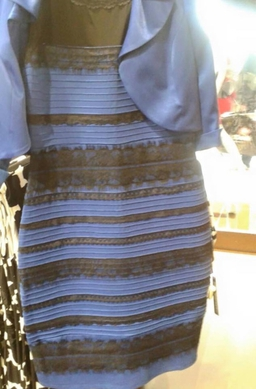
\includegraphics{../images/the_dress.jpg}

}

\caption{From the wikipedia page: The dress}

\end{figure}
\end{frame}

\begin{frame}{The Dress}
\protect\hypertarget{the-dress}{}
\begin{itemize}[<+->]
\tightlist
\item
  Is that too long ago to be a pop culture example still?
\item
  Anyway, apparently it looks different to different people.
\end{itemize}
\end{frame}

\begin{frame}{Five Theories}
\protect\hypertarget{five-theories}{}
\begin{enumerate}[<+->]
\tightlist
\item
  Eliminativism
\item
  Subjectivism
\item
  Potential
\item
  Physical
\item
  Strong Realism
\end{enumerate}
\end{frame}

\begin{frame}{Eliminativism}
\protect\hypertarget{eliminativism}{}
There are no colors!

\begin{itemize}[<+->]
\tightlist
\item
  Downsides: Not really consistent with how we talk.
\item
  Upsides: Don't have the problem of fitting colors into a physical
  world.
\end{itemize}
\end{frame}

\begin{frame}{Objects aren't Colored}
\protect\hypertarget{objects-arent-colored}{}
From our perspective, the following view is similar.

\begin{itemize}[<+->]
\tightlist
\item
  Light is colored, or at least some light is.
\item
  But no objects are.
\item
  Maybe we can talk about blue chairs, but chairs are never literally
  blue.
\end{itemize}
\end{frame}

\begin{frame}{Still Strange}
\protect\hypertarget{still-strange}{}
This has some metaphysical advantages, but it's a mess as a theory of
perception.

\begin{itemize}[<+->]
\tightlist
\item
  It looks like objects are colored.
\item
  If you say they aren't, and that it's just a figure of speech to say
  they are, you can \textbf{maybe} rescue accuracy, but you've given up
  fidelity.
\end{itemize}
\end{frame}

\begin{frame}{Subjectivism}
\protect\hypertarget{subjectivism}{}
Everything is exactly how it seems.

\begin{itemize}[<+->]
\tightlist
\item
  If it seems different to you and to me, things are different for you
  and for me.
\item
  The dress might be blue for one person, and white for another.
\end{itemize}
\end{frame}

\begin{frame}{Fidelity}
\protect\hypertarget{fidelity}{}
Is this high fidelity?

\begin{itemize}[<+->]
\tightlist
\item
  Probably not; it seems like we are seeing things as they are.
\item
  That's why people thought they were \textbf{disagreeing} about the
  dress.
\end{itemize}
\end{frame}

\begin{frame}{Disagreement}
\protect\hypertarget{disagreement}{}
On the subjectivist view, it's like the disagreement when one person
says ``I grew up in Michigan'' and another says ``I didn't.''
\end{frame}

\begin{frame}{Potential}
\protect\hypertarget{potential}{}
To say that something is red is not to say that I see it as red, but
that it has the potential to cause red experiences.

\begin{itemize}[<+->]
\tightlist
\item
  As Pasnau a few times alludes to, this is the natural theory of humor.
\item
  To say that a joke is funny just is to say that it has the potential
  to make (typical) people laugh.
\end{itemize}
\end{frame}

\begin{frame}{What Potential}
\protect\hypertarget{what-potential}{}
Anything \emph{could} look red if you shine a strong enough red light on
it.

\begin{itemize}[<+->]
\tightlist
\item
  It has to be that red things are red looking in normal enough
  conditions.
\item
  If normal enough means that some normal people see it that way, I
  think the dress turns out to be both blue and white.
\end{itemize}
\end{frame}

\begin{frame}{Too Subjective}
\protect\hypertarget{too-subjective}{}
Do colors look like things that are less about us?

\begin{itemize}[<+->]
\tightlist
\item
  I don't know; when you find a joke funny does that seem like less an
  objective feature of reality than when you find a dress blue?
\end{itemize}
\end{frame}

\begin{frame}{Causal}
\protect\hypertarget{causal}{}
Intuitively, something looks red because it is red.

\begin{itemize}[<+->]
\tightlist
\item
  On this view, something is red because it looks red.
\item
  Should we worry about that? Maybe, and that motivates the next view.
\end{itemize}
\end{frame}

\begin{frame}{Physical}
\protect\hypertarget{physical}{}
The main point of this whole part of the lecture is to distinguish 3 and
4.

\begin{enumerate}[<+->]
\tightlist
\item
  Eliminativism
\item
  Subjectivism
\item
  Potential
\item
  \textbf{Physical}
\item
  Strong Realism
\end{enumerate}
\end{frame}

\begin{frame}{Physical}
\protect\hypertarget{physical-1}{}
On what I'm calling `physical' views, colors are identified with the
physical things that make them appear to have the color they do.

\begin{itemize}[<+->]
\tightlist
\item
  The moderns thought that was something about rotation.
\end{itemize}
\end{frame}

\begin{frame}{Physical}
\protect\hypertarget{physical-2}{}
On what I'm calling `physical' views, colors are identified with the
physical things that make them appear to have the color they do.

\begin{itemize}[<+->]
\tightlist
\item
  In fact it's something about which wavelengths of light get absorbed
  or reflected. It is microphysical like they thought, but the mechanism
  is the same.
\end{itemize}
\end{frame}

\begin{frame}{Good Features}
\protect\hypertarget{good-features}{}
\begin{itemize}[<+->]
\tightlist
\item
  Colors cause color experiences.
\item
  Colors are in the world.
\end{itemize}
\end{frame}

\begin{frame}{Bad Features}
\protect\hypertarget{bad-features}{}
\begin{itemize}[<+->]
\tightlist
\item
  Still a challenge with describing which physical characteristics. The
  ones that cause red experiences for \emph{who}, and \emph{in what
  circumstances}.
\item
  Horrible on fidelity; colors don't look like surface reflectance
  characteristics.
\end{itemize}
\end{frame}

\begin{frame}{Strong Realism}
\protect\hypertarget{strong-realism}{}
\begin{itemize}[<+->]
\tightlist
\item
  So one last theory: colors are real, and they are the way they seem.
\item
  Very hard to square this with a broadly materialist world!
\item
  I'm mostly going to set this aside, but if you really want fidelity!
\end{itemize}
\end{frame}

\begin{frame}{For Next Time}
\protect\hypertarget{for-next-time}{}
Onto chapter 4, where we talk about introspection as the place for
optimism.
\end{frame}



\end{document}
